\chapter{Method}
\label{chapter:method}
\epigraph{\textit{Du bist schön, aber dafür kannst du nichts.
Weder Lesen, noch Schreiben, noch was anderes}}{Alligatoah}
With the theory discussed in the previous chapter it is now possible to build a model for numerical simulations.
Numerical simulations have been at the heart of fluid dynamics for a long time.
This is mainly because of two statements.
On the one hand we can not find an analytical solution to any given flow problem, that has to do with the shape and structure of the Navier-Stokes equations.
In fact there are only a few analytical solutions known. 
They are often referred to as benchmark problems.
One of those is the famous ''Hagen–Poiseuille law'' which is an analytical solution for a flow field in a canal and was first derived by Poiseuille and Haagen in the 18th century~\cite{sutera1993history}.

On the other hand solving differential equations with numerical tools is a story of success.
Long before any computer was build, iterative methods for approximating a solution to a given differential or integral equation have been developed.
With Leonhard Euler pulished what we call the ''Euler-method'' already in the 18th century~\cite{brezinski2012numerical}.
On the brink to the 20th century Carl Runge and Martin Kutta developed the method nowadays called ''Runge-Kutta'' which is numerically better than a plain Euler solver.

Several physics problems are being studied almost exclusively with numerical tools.
Computational fluid dynamics (CFD) is one of those fields.
Although Moors law has been broken for a few years the computing power is still growing rapidly~\cite{591665}.
Of course instead of ever fast processors, the trend goes in the direction of parallel computing and accelerated computing with accelerator devices such as graphic processing units (GPUs).
While a GPU lacks the complexity of a CPU it excels at doing simple task over and over again.
For example generate a single colorful pixel for as output for a monitor.
As it turns out the lattice Boltzmann method is well suited to be calculated on the GPU, there are of course limitations that will be discussed later.

In the following of this chapter a short overview of numerical methods to simulate the thin film equation will be given.
After the short overview the lattice Boltzmann method will be introduced, first from a mathematical perspective with it's link to kinetic theory and later from the numerical point of view.
This chapter will end with some examples proofing that the lattice Boltzmann method as presented here is indeed able to simulate the behaviour of thin liquid film.

\section{Numerical Methods}\label{sec:numerical_methods}
\begin{figure}
    \centering
    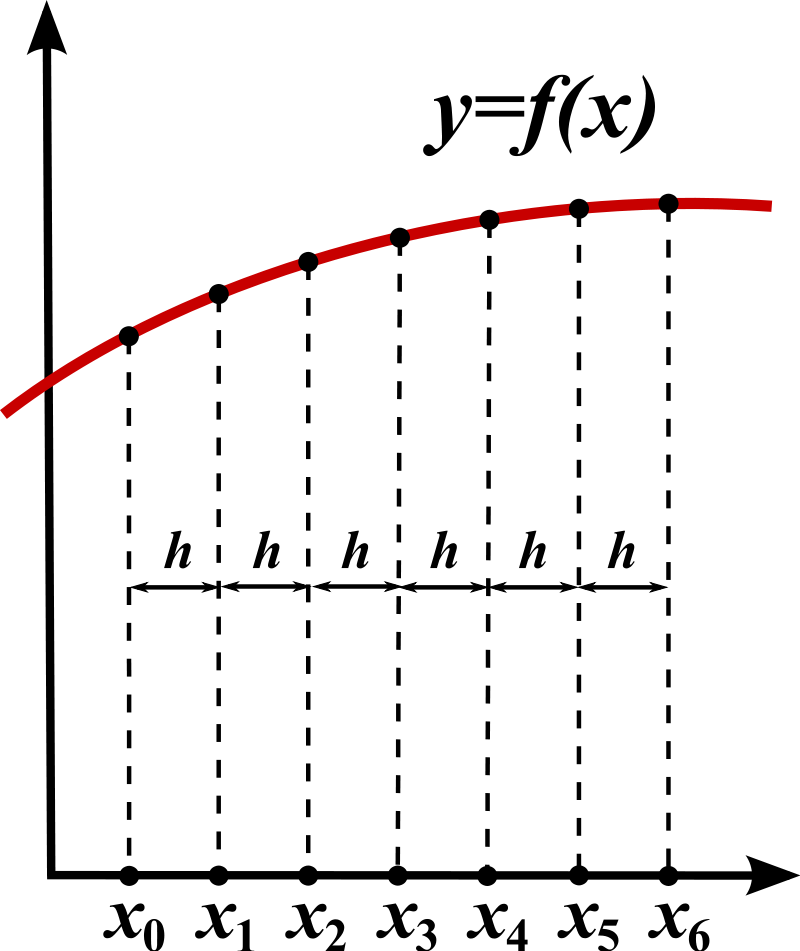
\includegraphics[width=0.5\textwidth]{graphics/800px-Finite_Differences.svg.png}
    \caption{Discretization of a continuous function y (in red) along a disrete space x.
    Each point is the disrete space of x is shifted by the distance h.
    Such the discrete function y of $x\in\{x_0, x_1, x_2, ...\}$ is a straight conection between the dots.}
    \label{fig:finite_difference}
\end{figure}
The lattice Boltzmann method is one among many to simulate the behaviour of a fluid.
Especially when it comes to numerical simulations of the thin film equation, other numerical approaches seem far more established and have been successfully applied for more then thirty years.
Since the thin film equation is a fourth order partial differential equation (PDE) one has to be careful in choosing an appropriate approach.
Careful in the sense that not every numerical scheme will be able to provide a correct solution.
This is for example the case when a simple Euler approach is used.
The problem is the fourth order differential in space and the non linear nature of the equation, see Eq.~\ref{eq:simple_thin_film}.
Still there are finite difference or element schemes that can be used to simulate the thin film equation.
Using finite differences or elements means nothing more that discretizing the continuous problem.
Concerning the thin film equation a rather well working scheme is the Crank-Nicolson scheme~\cite{crank_nicolson_1947, PhysRevE.63.011208, 10.5555/1403886}, dr discontinous Galerkin methods~\cite{ern2013theory}.
However all finite difference or element schemes suffer from the concrete choice of discretization, which is often referred as discritization artifacts.
Since the starting equation is usually defined in continuous space and time one needs to discretize the system, i.e. introduce a lattice for both the space and the time to make the problem appropriate for computation. 
For example take a sine wave and mark two points along the curve.
Connecting them will not show the sine wave but a straight line.
Increasing the number of points along the curve will increase the accuracy of the resulting approximation as displayed in Fig.\ref{fig:finite_difference}.
To understand that this curve is a sine at least a few more points are needed.
Which explains the so called fidelity of the finite difference method.
One needs a fine enough grid to resolve the important dynamics, but the smaller the lattice spacing gets the more numerically demanding is the algorithm.
In fact there are further limitations to the problem of numerically solving a PDE.
For PDEs in generell, like the thin film equation, one needs to statisfy the Courant–Friedrichs–Lewy condition (CFL)~\cite{courant1928partiellen}.  
Which beyond other things states that choosing a increment for time can not be independent of the increment for space.
This can be written as
\begin{equation}\label{eq:CFL}
    C = \Delta t \left(\sum_{i=1}^n \frac{u_{x_i}}{\Delta x_i}\right) \leq C_{max},
\end{equation}
with $\Delta x$ and $\Delta t$ being the spatial and temporal increment, respectively and  $u_{x_i}$ being the magnitude of the velocity in the respective direction.
Behind this concept is the idea that a given wave should not propagate from lattice point to lattice point, but should perform several iterations between two lattice points.
$C_{max}$ is one for an explicit solver, like the vanilla lattice Boltzmann method.
But can be relaxed to be larger than one for implicit methods.

Of course it is as well possible to perform a transformation and solve the differential equation in Fourier space, or in other words perform a Fourier Transformation (FT).
The set of solvers using a FT to solve a given differential equation is called spectral methods.
Doing so has the advantage of interchanging the derivatives with simple multiplications.
For example the term $\partial_x f(x)$ transforms to  
\begin{equation}\label{eq:fourier_transform}
    \partial_x f(x) = k\cdot \tilde{f}(k).
\end{equation}
Thus instead of solving a differential equation one just has to solve an algebraic equation, or a set of algebraic equations.
One problem however is the backward transformation. 
Usually the expressions are fairly complicated and often the backward transformation into real space is not easy to perform.
Since this is a transformation an operator for the transformation is needed.
These operators are usually matrices, which depend on the explicit problem.
To get a solution it is often needed to invert these operators, which by far a non trivial numerical task.
Nevertheless these transformation approaches are often quite helpful finding an exact solution.
One rather prominat example is the computation of Green's functions.

\section{The Lattice Boltzmann Method}\label{sec:LBM}
The reason why the lattice Boltzmann method is lacking behind when it comes to thin films is that the method in principle always approximated the Navier-Stokes equations.
However the lattice Boltzmann method has strong ties with the CDF community.
Due the simplicity of the method a lot has been worked out over last fourty years.
Since the method got first developed in the 1986 it has gained more and more popularity~\cite{PhysRevLett.56.1505}.

In the first iteration of the lattice Boltzmann method it was yet unclear how many velocities were needed to approximate the Navier-Stokes equations.

\begin{equation}\label{eq:LBM_discret_noforces}
    f_{\alpha}(\mathbf{x}+\mathbf{c}_{\alpha}\Delta t, t+ \Delta t) - f_{\alpha}(\mathbf{x}, t) = \frac{1}{\tau}(f^{eq}_{\alpha}(\mathbf{x}, t)-f_{\alpha}(\mathbf{x}, t)).
\end{equation}

\begin{equation}\label{eq:weightsD1Q3}
w_{\alpha} = \begin{cases}
2/3 &\text{$\alpha = 0$}\\
1/6 &\text{$\alpha = 1$}\\
1/6 &\text{$\alpha = 2$}
\end{cases}
\end{equation}



\begin{equation}\label{eq:weightsD2Q9}
w_{\alpha} = \begin{cases}
4/9 &\text{$\alpha = 0$}\\
1/9 &\text{$\alpha = 1,2,3,4$}\\
1/36 &\text{$\alpha = 5,6,7,8$}
\end{cases}
\end{equation}

\subsection{Lattice Boltzmann for shallow water problems}

\begin{gather}\label{eq:equilibria_D1Q3}
    f_{0}^{eq} = h\left(1-\frac{1}{2c}gh - \frac{1}{c^2}u^2\right)\nonumber\\
    f_{1}^{eq} = h\left(\frac{1}{2c}gh + \frac{1}{2c}u - \frac{1}{c^2}u^2\right)\\
    f_{2}^{eq} = h\left(1-\frac{1}{2c}gh + \frac{1}{2c}u - \frac{1}{c^2}u^2\right)\nonumber
\end{gather}

\begin{equation}\label{eq:equilibria_D2Q9}
    f_{\alpha}^{eq} =\begin{cases} 
    h + w_{\alpha}h\left(-\frac{15}{8}gh - \frac{3}{2}\mathbf{u}^2\right) &\text{$\alpha = 0$}\\
    w_{\alpha}h\Big(\frac{3}{2}gh + 3~\mathbf{c}_{\alpha}\cdot\mathbf{u} + \frac{9}{2}(\mathbf{c}_{\alpha}\cdot\mathbf{u}) - \frac{3}{2}\mathbf{u}^2\Big) &\text{$\alpha \ne 0$}
    \end{cases}
\end{equation}

\subsection{Thin film flows}


\begin{equation}\label{eq:force_slip}
    \alpha_{\delta}(h) = \frac{6h}{2h^2+6h\delta + 3\delta^2}
\end{equation}


\begin{equation}\label{eq:disjoining_pressure}
    \Pi(h) = \kappa f(h) = \gamma(1-\cos(\theta))\frac{(n-1)(m-1)}{(n-m)h_{\ast}}\left[\left(\frac{h_{\ast}}{h}\right)^n-\left(\frac{h_{\ast}}{h}\right)^m\right].
\end{equation}